\section{Metodología}
    El primer paso a realizar en esta investigación es recrear el código mostrado en \cite{Bullinaria2009}, donde se describe la implementción de una red  neuronal multi capa usando el algoritmo de entrenamiento backpropagation en le lenguaje de programación Python.  Para esto se utilizará el conjunto de datos de Optical Digits,  en donde se tendrá que preprocesar los datos, para eliminar registros invalidos. 

    Posteriormente se implementará una nueva versión del código en donde se experimentará con mas de dos capas de pesos duplicados para mejorar la tasa de olvido de infromación al momento de usar el aprendizaej incremental.  Para ello se explorará incrementando gradualmente el nueron de capas de pesos duplicados, hasta llega un punto que mas capas no generen un decremento de las tasas de olvido/error.

(Revisen la redacción y mejorenla de favor)
    Cuando los dos proyectos se tengan, se realizar\'a una comparación, donde se vera cual de estos dos experimentos
    es más eficaz en proyectos de la vida real.
    
\section{Cronograma de Actividades}
(El cronograma de actividades dice John Bullinaria en la parte de arriba, eliminar eso)

    \begin{figure}[H]
        \centering
        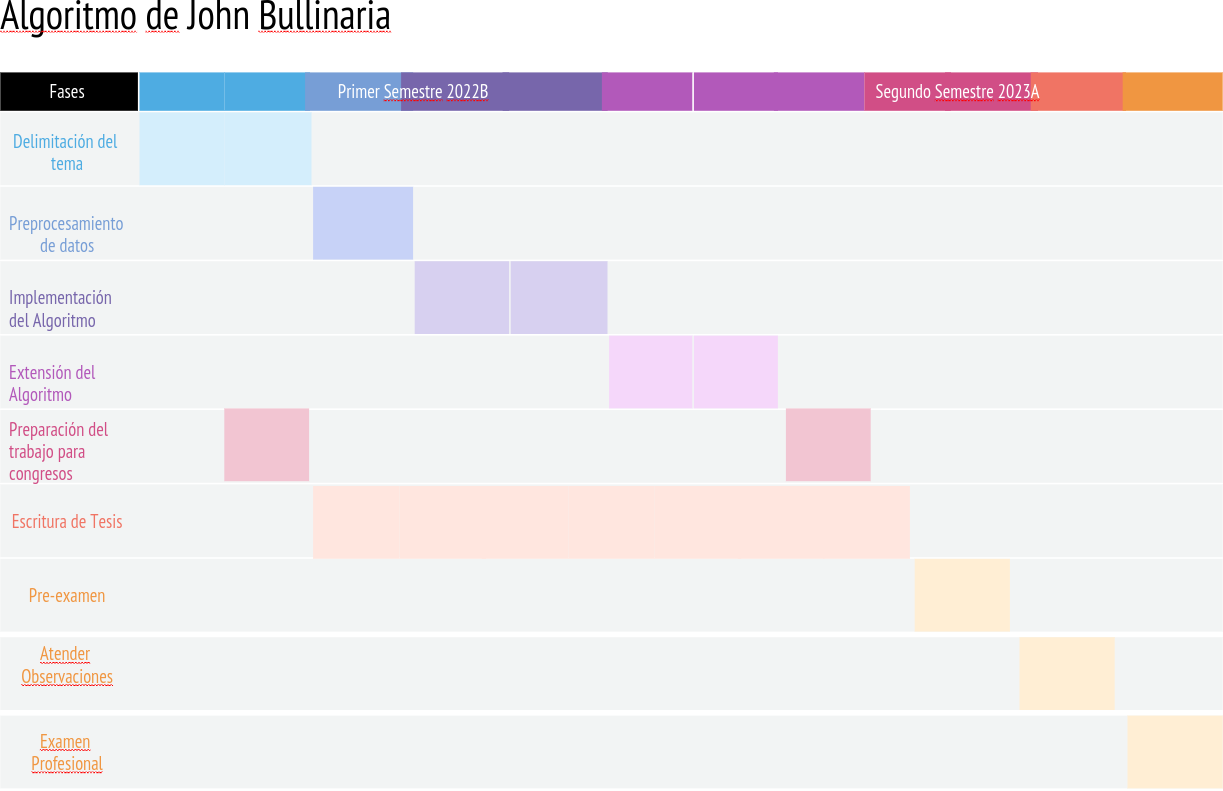
\includegraphics[width=\columnwidth]{diagramaGantt.png}
        %\caption{Elimine estoa horita, no hace falta ponerle un titulo, dado que es la únic figura en la sección}
        \label{fig:fig3}
    \end{figure}

\section{Organización del Capitulado}


	En el capitulo 2 se ver\'a lo que es el aprendizaje humano y el aprendizaje incremental con sus algoritmos, se describirán las redes neuronales artificiales.

En el capitulo 3 se implementar\'a el articulo de John A. Bullinaria, como funciona, resultado que da al pasar los datos que dice para comprobar que funciona como menciona en su art\'iculo. En el capitulo 4 se explicar\'a como se hará la modificación a su algoritmo, cuantas capas se van a poner, como se van a repartir las tazas de aprendizaje.

Posteriormente en el capitulo 5 se mostrar\'a una comparación de los resultados de ambos trabajos. En el capitulo 6 se verán las conclusiones y trabajo futuro.
